\documentclass[11pt,a4paper]{article}
\usepackage[utf8]{inputenc}
\usepackage[vietnamese]{babel}
\usepackage{amsmath,amssymb}
\usepackage[version=4]{mhchem}
\usepackage{geometry}
\geometry{top=1.5cm,bottom=1.2cm,left=1.4cm,right=1.4cm,headheight=28pt,headsep=12pt,footskip=18pt}
\usepackage{graphicx}
\usepackage{xcolor}
\usepackage{tabularx}
\usepackage{array}
\usepackage{tikz}
\usepackage{fancyhdr}
\usepackage{enumitem}
\usepackage{multido}
\usepackage{tcolorbox}
\usepackage{colortbl}

\definecolor{hfRed}{HTML}{D32F2F}
\definecolor{hfGreen}{HTML}{8BC390}
\definecolor{mainGreen}{HTML}{2E7D32}
\definecolor{solBlue}{HTML}{1565C0}
\definecolor{tableGreen}{HTML}{E8F5E9}

\usepackage{ex_test}

\pagestyle{fancy}
\fancyhf{}
\renewcommand{\headrulewidth}{0.75pt}
\renewcommand{\headrule}{\hbox to\headwidth{\color{hfGreen}\leaders\hrule height \headrulewidth\hfill}}
\renewcommand{\footrulewidth}{0.75pt}
\renewcommand{\footrule}{\hbox to\headwidth{\color{hfGreen}\leaders\hrule height \footrulewidth\hfill}}

\fancyhead[L]{\small\itshape\color{hfRed}Tài liệu lưu hành nội bộ}
\fancyhead[R]{\small\color{hfRed}Thầy \textbf{TRẦN VĂN THẠNH} - 0777.470.803}

\fancyfoot[L]{\footnotesize\itshape\color{hfRed}CS1: 6/15 Nguyễn Hoàng, P. Kim Long, TP Huế \quad|\quad CS2: 24 Đặng Thái Thân, TP Huế}
\fancyfoot[R]{\small\textbf{\color{hfRed}Trang \thepage}}

\setlength{\parindent}{0pt}
\setlength{\parskip}{2pt}

\begin{document}

\begin{minipage}[t]{0.45\textwidth}
\textbf{TỔ LÍ - HÓA}\\
\textbf{ĐỀ CHÍNH THỨC}\\
\textit{(Đề thi có 04 trang)}
\end{minipage}
\hfill
\begin{minipage}[t]{0.52\textwidth}
\raggedleft
\textbf{\color{hfRed}ĐỀ KIỂM TRA GIỮA HỌC KÌ I}\\
\textbf{MÔN: HOÁ HỌC -- LỚP 10}\\
\textit{Thời gian làm bài: 45 phút (không kể thời gian phát đề)}\\
\textbf{MÃ ĐỀ THI: 1201}
\end{minipage}

\vspace{4pt}
\noindent
\textit{Họ và tên thí sinh:} \dotfill \textit{SBD:} \dotfill

\vspace{2pt}
\noindent
\textit{\footnotesize (Cho biết nguyên tử khối: $\ce{H=1; B=10,81; C=12; N=14; O=16; F=19; Ne=20,19; Na=23; Mg=24; P=31; S=32; Cl=35,5; K=39; Ca=40; Fe=56; Br=79,91}$).}

\vspace{2pt}
\begin{center}
\textbf{CHÚ Ý: Học sinh không được sử dụng bảng tuần hoàn các nguyên tố hóa học.}
\end{center}

\vspace{2pt}
\hrule color{hfGreen} height 0.5pt

\vspace{4pt}
\begin{center}
\textbf{\color{hfRed}\large (BẢN GIÁO VIÊN -- CÓ LỜI GIẢI CHI TIẾT)}
\end{center}

\vspace{2pt}
\begin{center}
{\color{hfRed}\textbf{\large BẢNG ĐÁP ÁN RÚT GỌN (DÀNH CHO GIÁO VIÊN)}}
\end{center}

\vspace{2pt}
\noindent
\textbf{\color{mainGreen}1. Phần I: Trắc nghiệm nhiều lựa chọn (3,0 điểm - mỗi câu đúng 0,25 điểm)}
\begin{center}
\renewcommand{\arraystretch}{1.2}
\begin{tabular}{|c|c|c|c|c|c|c|c|c|c|c|c|c|}
\hline
\rowcolor{tableGreen}
\textbf{Câu} & \textbf{1} & \textbf{2} & \textbf{3} & \textbf{4} & \textbf{5} & \textbf{6} & \textbf{7} & \textbf{8} & \textbf{9} & \textbf{10} & \textbf{11} & \textbf{12} \\
\hline
\textbf{Đ/A} & \textbf{\color{hfRed}B} & \textbf{\color{hfRed}A} & \textbf{\color{hfRed}A} & \textbf{\color{hfRed}C} & \textbf{\color{hfRed}D} & \textbf{\color{hfRed}C} & \textbf{\color{hfRed}C} & \textbf{\color{hfRed}C} & \textbf{\color{hfRed}B} & \textbf{\color{hfRed}C} & \textbf{\color{hfRed}B} & \textbf{\color{hfRed}A} \\
\hline
\end{tabular}
\end{center}

\vspace{2pt}
\noindent
\textbf{\color{mainGreen}2. Phần II: Trắc nghiệm Đúng / Sai (2,0 điểm)}
\begin{center}
\renewcommand{\arraystretch}{1.2}
\begin{tabular}{|c|c|c|c|c|}
\hline
\rowcolor{tableGreen}
\textbf{Câu} & \textbf{Lệnh a)} & \textbf{Lệnh b)} & \textbf{Lệnh c)} & \textbf{Lệnh d)} \\
\hline
\textbf{Câu 1} & \textbf{\color{hfRed}ĐÚNG} & \textbf{\color{solBlue}SAI} & \textbf{\color{solBlue}SAI} & \textbf{\color{hfRed}ĐÚNG} \\
\hline
\textbf{Câu 2} & \textbf{\color{hfRed}ĐÚNG} & \textbf{\color{solBlue}SAI} & \textbf{\color{solBlue}SAI} & \textbf{\color{solBlue}SAI} \\
\hline
\end{tabular}
\end{center}

\vspace{2pt}
\noindent
\textbf{\color{mainGreen}3. Phần III: Trả lời ngắn (2,0 điểm - mỗi câu đúng 0,5 điểm)}
\begin{center}
\renewcommand{\arraystretch}{1.2}
\begin{tabular}{|c|c|c|c|c|}
\hline
\rowcolor{tableGreen}
\textbf{Câu} & \textbf{Câu 1} & \textbf{Câu 2} & \textbf{Câu 3} & \textbf{Câu 4} \\
\hline
\textbf{Đáp án} & \textbf{\color{hfRed}58} & \textbf{\color{hfRed}4} & \textbf{\color{hfRed}2} & \textbf{\color{hfRed}1} \\
\hline
\end{tabular}
\end{center}

\vspace{4pt}
\hrule color{hfGreen} height 0.5pt

\vspace{4pt}
\noindent
{\color{mainGreen}\textbf{\Large A. PHẦN TRẮC NGHIỆM (7 ĐIỂM)}}

\vspace{3pt}
\noindent
{\color{mainGreen}\textbf{\large PHẦN I. Câu trắc nghiệm nhiều phương án lựa chọn (3,0 điểm)}}\\
\textit{\small Thí sinh trả lời từ câu 1 đến câu 12. Mỗi câu hỏi thí sinh chỉ chọn một phương án.}
\vspace{2pt}

\begin{ex}
Đường kính của nguyên tử khoảng $10^2\text{ pm}$, trong khi đường kính của hạt nhân khoảng $10^{-2}\text{ pm}$. Đường kính nguyên tử lớn gấp bao nhiêu lần so với đường kính hạt nhân?
\choice
{1000.}
{\True 10000.}
{100.}
{10.}

\loigiai{
Tỉ số giữa đường kính của nguyên tử và đường kính của hạt nhân là:
$$\frac{d_{\text{nguyên tử}}}{d_{\text{hạt nhân}}} = \frac{10^2}{10^{-2}} = 10^{2 - (-2)} = 10^4 = 10\,000\text{ (lần)}.$$
\textbf{Chọn B.}
}
\end{ex}
\begin{ex}
Số electron tối đa có trong 1 AO p là
\choice
{\True 2.}
{6.}
{3.}
{1.}

\loigiai{
Theo nguyên lí Pauli, trong mỗi một orbital nguyên tử (AO) chỉ chứa tối đa 2 electron có chiều tự quay khác nhau.\\
Phân lớp p gồm 3 AO p nên chứa tối đa 6 electron, còn mỗi 1 AO p chỉ chứa tối đa 2 electron.\\
\textbf{Chọn A.}
}
\end{ex}
\begin{ex}
Phát biểu nào sau đây không đúng khi nói về vai trò của hóa học đối với đời sống và sản xuất?
\choice
{\True Nghiên cứu quy luật hình thành, vận động của các thiên thể và địa tầng Trái Đất.}
{Cung cấp phân bón hóa học và thuốc bảo vệ thực vật nhằm tăng năng suất nông nghiệp.}
{Nghiên cứu và sản xuất các loại thuốc chữa bệnh, vắc-xin và vật tư y tế.}
{Tạo ra các sản phẩm tiêu dùng thiết yếu như xà phòng, chất tẩy rửa và chất dẻo.}

\loigiai{
- Nghiên cứu quy luật hình thành, vận động của các thiên thể thuộc về Thiên văn học; nghiên cứu địa tầng Trái Đất thuộc về Địa chất học.\\
- Các phát biểu B, C, D đều thể hiện đúng vai trò thiết thực của Hóa học trong nông nghiệp, y học và đời sống.\\
\textbf{Chọn A.}
}
\end{ex}
\begin{ex}
X là nguyên tố s. Trong bảng tuần hoàn, X có thể thuộc nhóm
\choice
{IB.}
{VIA.}
{\True IA.}
{VIB.}

\loigiai{
Nguyên tố s là các nguyên tố mà nguyên tử có electron cuối cùng được điền vào phân lớp s. Trong bảng tuần hoàn, các nguyên tố s thuộc nhóm IA hoặc IIA (và He ở nhóm VIIIA). Trong các phương án đề bài cho, chỉ có nhóm IA là phù hợp.\\
\textbf{Chọn C.}
}
\end{ex}
\begin{ex}
Trong bảng tuần hoàn các nguyên tố hóa học do nhà hóa học người Nga D. I. Mendeleev (1834 -- 1907) đề xuất năm 1869, các nguyên tố được sắp xếp theo chiều tăng dần của
\choice
{số hiệu nguyên tử.}
{số electron hóa trị.}
{bán kính nguyên tử.}
{\True khối lượng nguyên tử.}

\loigiai{
Năm 1869, Mendeleev đã sắp xếp các nguyên tố hóa học theo chiều tăng dần của khối lượng nguyên tử (nguyên tử khối). Bảng tuần hoàn hiện đại sau này mới sắp xếp theo chiều tăng dần của điện tích hạt nhân (số hiệu nguyên tử).\\
\textbf{Chọn D.}
}
\end{ex}
\begin{ex}
Bảng tuần hoàn các nguyên tố hóa học hiện nay gồm có
\choice
{6 chu kì và 16 nhóm.}
{8 chu kì và 18 nhóm.}
{\True 7 chu kì và 18 cột.}
{7 chu kì và 8 nhóm.}

\loigiai{
Bảng tuần hoàn hiện đại gồm có 7 chu kì (được đánh số từ 1 đến 7) và 18 cột (ứng với 8 nhóm A và 8 nhóm B gồm 16 nhóm).\\
\textbf{Chọn C.}
}
\end{ex}
\begin{ex}
Hạt mang điện trong hạt nhân nguyên tử là
\choice
{neutron và electron.}
{electron.}
{\True proton.}
{neutron.}

\loigiai{
Hạt nhân nguyên tử gồm hai loại hạt: proton (mang điện tích dương $+1$) và neutron (không mang điện). Do đó hạt mang điện trong hạt nhân chỉ có proton.\\
\textbf{Chọn C.}
}
\end{ex}
\begin{ex}
Cho các phát biểu về sự chuyển động của electron trong nguyên tử như sau:\\
(a) Theo mô hình hành tinh nguyên tử, các electron chuyển động xung quanh hạt nhân theo những quỹ đạo tròn hay bầu dục.\\
(b) Theo mô hình hiện đại, các electron chuyển động rất nhanh xung quanh hạt nhân theo một quỹ đạo xác định tạo thành đám mây electron.\\
(c) Theo mô hình hiện đại, trong nguyên tử, electron chuyển động rất nhanh, không theo quỹ đạo xác định.\\
(d) Theo mô hình hiện đại, xác suất tìm thấy electron tại mỗi điểm trong không gian của AO là 90\%.\\
Số phát biểu đúng là
\choice
{1.}
{4.}
{\True 2.}
{3.}

\loigiai{
- (a) \textbf{Đúng}: Theo mô hình Rutherford -- Bohr, electron chuyển động quanh hạt nhân theo những quỹ đạo xác định tròn hay elip.\\
- (b) \textbf{Sai}: Mô hình hiện đại khẳng định electron chuyển động không theo quỹ đạo xác định.\\
- (c) \textbf{Đúng}: Theo mô hình hiện đại, electron chuyển động rất nhanh và không theo quỹ đạo xác định nào.\\
- (d) \textbf{Sai}: Orbital nguyên tử (AO) là khu vực không gian xung quanh hạt nhân mà tại đó xác suất tìm thấy electron là khoảng 90\%, chứ không phải tại mỗi điểm trong không gian xác suất đều là 90\%.\\
Có 2 phát biểu đúng là (a) và (c).\\
\textbf{Chọn C.}
}
\end{ex}
\begin{ex}
Trong nguyên tử, vùng không gian bao quanh hạt nhân và mang điện tích âm được tạo nên bởi các hạt
\choice
{proton.}
{\True electron.}
{neutron.}
{alpha.}

\loigiai{
Lớp vỏ nguyên tử mang điện tích âm bao quanh hạt nhân được cấu tạo từ các hạt electron ($e$).\\
\textbf{Chọn B.}
}
\end{ex}
\begin{ex}
Kí hiệu phân lớp electron nào sau đây không đúng?
\choice
{3p.}
{3s.}
{\True 3f.}
{3d.}

\loigiai{
Lớp thứ 3 ($n = 3$) chỉ gồm 3 phân lớp là $3s, 3p, 3d$. Phân lớp $f$ chỉ xuất hiện từ lớp thứ 4 trở đi ($4f, 5f,\dots$). Do đó kí hiệu $3f$ là không đúng.\\
\textbf{Chọn C.}
}
\end{ex}
\begin{ex}
Phát biểu nào sau đây không đúng?
\choice
{Khối lượng hạt electron nhỏ hơn nhiều so với khối lượng hạt proton.}
{\True Khối lượng nguyên tử tập trung chủ yếu ở lớp vỏ.}
{Trong nguyên tử, khối lượng tập trung chủ yếu ở hạt nhân.}
{Hạt proton và hạt neutron có khối lượng gần bằng nhau.}

\loigiai{
Vì khối lượng của electron rất bé ($m_e \approx 0,00055\text{ amu}$) so với proton và neutron ($m_p \approx m_n \approx 1\text{ amu}$), khối lượng nguyên tử tập trung hầu như hoàn toàn ở hạt nhân. Phát biểu B cho rằng khối lượng tập trung ở lớp vỏ là sai.\\
\textbf{Chọn B.}
}
\end{ex}
\begin{ex}
Cho các nguyên tử: $^{12}_6\ce{X}, ^{14}_7\ce{Y}, ^{14}_6\ce{Z}, ^{24}_{12}\ce{T}$. Các nguyên tử thuộc cùng một nguyên tố hóa học là
\choice
{\True \ce{X} và \ce{Z}.}
{\ce{X} và \ce{T}.}
{\ce{Y} và \ce{Z}.}
{\ce{Z} và \ce{T}.}

\loigiai{
Nguyên tố hóa học là tập hợp các nguyên tử có cùng số đơn vị điện tích hạt nhân (cùng số proton $Z$).\\
Ta thấy $^{12}_6\ce{X}$ và $^{14}_6\ce{Z}$ đều có $Z = 6$ (nguyên tố Carbon - $\ce{C}$) nên thuộc cùng một nguyên tố hóa học.\\
\textbf{Chọn A.}
}
\end{ex}
\vspace{4pt}
\noindent
{\color{mainGreen}\textbf{\large PHẦN II. Câu trắc nghiệm đúng sai (2,0 điểm)}}\\
\textit{\small Thí sinh trả lời từ câu 1 đến câu 2. Trong mỗi ý a), b), c), d) ở mỗi câu, thí sinh chọn đúng hoặc sai.}
\vspace{2pt}

\begin{ex}
Fluorine và hợp chất của nó được sử dụng làm chất chống sâu răng, chất cách điện, chất làm lạnh, vật liệu chống dính, \dots\ Nguyên tử fluorine (\ce{F}) chứa 9 electron và có số khối là 19.
\choiceTF
{\True Hạt nhân nguyên tử \ce{F} có 9 proton và 10 neutron}
{Nguyên tử \ce{F} có điện tích lớp vỏ là +9}
{Khối lượng của một nguyên tử \ce{F} xấp xỉ 28 amu}
{\True Phân tử $\ce{RF2}$ có tổng số hạt mang điện là 60. Nguyên tử của nguyên tố R có 2 electron thuộc lớp M và R là nguyên tố kim loại}

\loigiai{
a) \textbf{ĐÚNG}: Nguyên tử \ce{F} có $Z = 9 \implies p = 9$; số neutron $N = A - p = 19 - 9 = 10$.\\
b) \textbf{SAI}: Điện tích lớp vỏ là do 9 electron tạo nên, mang điện tích âm $-9$ (hoặc $-9e = -14,418 \cdot 10^{-19}\text{ C}$), không phải $+9$.\\
c) \textbf{SAI}: Khối lượng nguyên tử xấp xỉ bằng số khối $A = 19\text{ amu}$ (không phải $28\text{ amu}$).\\
d) \textbf{ĐÚNG}: Trong phân tử $\ce{RF2}$:\\
Tổng số hạt mang điện là $2Z_R + 2(2Z_{\ce{F}}) = 2Z_R + 36 = 60 \implies 2Z_R = 24 \implies Z_R = 12$ (Magnesium - $\ce{Mg}$).\\
Cấu hình electron của R: $\ce{1s^2 2s^2 2p^6 3s^2}$.\\
Lớp M ($n = 3$) có 2 electron ($3s^2$). Nguyên tử có 2 electron lớp ngoài cùng nên là kim loại.
}
\end{ex}
\begin{ex}
Boron (\ce{B}) là nguyên tố có nhiều tác dụng đối với cơ thể người như: làm lành vết thương, điều hoà nội tiết sinh dục, chống viêm khớp, \dots\ Do ngọn lửa cháy có màu đặc biệt nên boron vô định hình được dùng làm pháo hoa. Boron có hai đồng vị là $^{10}_5\ce{B}$ và $^{11}_5\ce{B}$, nguyên tử khối trung bình là 10,81.
\choiceTF
{\True Hai đồng vị của boron có cùng số proton nhưng khác nhau về số neutron}
{Nguyên tố \ce{B} thuộc chu kì 3 trong bảng tuần hoàn}
{Nguyên tử của nguyên tố \ce{B} có 4 electron s và có 3 electron ở phân lớp ngoài cùng}
{Phần trăm số nguyên tử của đồng vị $^{10}_5\ce{B}$ trong tự nhiên là 81\%}

\loigiai{
a) \textbf{ĐÚNG}: Các đồng vị của cùng một nguyên tố luôn có cùng số proton ($Z = 5$) nhưng khác nhau về số neutron ($^{10}_5\ce{B}$ có 5 neutron; $^{11}_5\ce{B}$ có 6 neutron).\\
b) \textbf{SAI}: Boron ($Z = 5$): $\ce{1s^2 2s^2 2p^1}$, có 2 lớp electron nên thuộc chu kì 2 (không phải chu kì 3).\\
c) \textbf{SAI}: Có 4 electron s ($1s^2 2s^2$). Nhưng phân lớp ngoài cùng là $2p$ chỉ có 1 electron (chứ không phải 3 electron ở phân lớp ngoài cùng; lớp ngoài cùng mới có 3 electron).\\
d) \textbf{SAI}: Gọi $x$ là \% số nguyên tử của $^{10}_5\ce{B}$:\\
$\frac{10x + 11(100 - x)}{100} = 10,81 \implies 1100 - x = 1081 \implies x = 19\%$.\\
Vậy $^{10}_5\ce{B}$ chiếm 19\%, còn $^{11}_5\ce{B}$ chiếm 81\%.
}
\end{ex}
\vspace{4pt}
\noindent
{\color{mainGreen}\textbf{\large PHẦN III. Câu trắc nghiệm yêu cầu trả lời ngắn (2,0 điểm)}}\\
\textit{\small Thí sinh trả lời từ câu 1 đến câu 4.}
\vspace{2pt}

\begin{ex}
Cho biết tổng số hạt proton, neutron và electron trong một nguyên tử của nguyên tố $^{39}_{19}\ce{K}$ là bao nhiêu?

\loigiai{
Trong nguyên tử $^{39}_{19}\ce{K}$:\\
- Số proton $p = 19$, số electron $e = 19$.\\
- Số neutron $n = A - p = 39 - 19 = 20$.\\
- Tổng số hạt: $S = p + e + n = 19 + 19 + 20 = 58$.\\
\textbf{Đáp án: 58.}
}
\end{ex}
\begin{ex}
Nguyên tử của nguyên tố calcium ($Z = 20$) có bao nhiêu lớp electron?

\loigiai{
Cấu hình electron của Calcium ($Z = 20$): $\ce{1s^2 2s^2 2p^6 3s^2 3p^6 4s^2}$.\\
Nguyên tử có 4 lớp electron ($n = 1, 2, 3, 4$).\\
\textbf{Đáp án: 4.}
}
\end{ex}
\begin{ex}
Cho các nguyên tử sau: $\ce{X}\ (Z = 11); \ce{Y}\ (Z = 17); \ce{Z}\ (Z = 20); \ce{T}\ (Z = 26)$. Có bao nhiêu nguyên tố thuộc loại nguyên tố s?

\loigiai{
Cấu hình electron:\\
- $\ce{X}\ (Z = 11)$: $\ce{1s^2 2s^2 2p^6 3s^1} \implies$ nguyên tố s.\\
- $\ce{Y}\ (Z = 17)$: $\ce{1s^2 2s^2 2p^6 3s^2 3p^5} \implies$ nguyên tố p.\\
- $\ce{Z}\ (Z = 20)$: $\ce{1s^2 2s^2 2p^6 3s^2 3p^6 4s^2} \implies$ nguyên tố s.\\
- $\ce{T}\ (Z = 26)$: $\ce{1s^2 2s^2 2p^6 3s^2 3p^6 3d^6 4s^2} \implies$ nguyên tố d.\\
Vậy có 2 nguyên tố s là $\ce{X}$ và $\ce{Z}$.\\
\textbf{Đáp án: 2.}
}
\end{ex}
\begin{ex}
Trong tự nhiên, nguyên tố bromine có 2 đồng vị là $^{79}_{35}\ce{Br}$ và $^{81}_{35}\ce{Br}$. Nguyên tử khối trung bình của bromine là 79,91. Trong hợp chất $\ce{NaBrO}_x$, nguyên tử đồng vị $^{81}\ce{Br}$ chiếm 30,994\% về khối lượng. Giá trị của $x$ là bao nhiêu (với O và Na là các đồng vị $^{16}_8\ce{O}, ^{23}_{11}\ce{Na}$)?

\loigiai{
Gọi $a$ là \% số nguyên tử của $^{79}\ce{Br}$ trong tự nhiên:\\
$\frac{79a + 81(100 - a)}{100} = 79,91 \implies 8100 - 2a = 7991 \implies a = 54,5\%$.\\
Tỉ lệ phần trăm số nguyên tử của $^{81}\ce{Br}$ là $100\% - 54,5\% = 45,5\%$ (ứng với tỉ lệ 0,455).\\
Trong 1 mol hợp chất $\ce{NaBrO}_x$:\\
$M = 23 + 79,91 + 16x = 102,91 + 16x\text{ (g/mol)}$.\\
Khối lượng đồng vị $^{81}\ce{Br}$: $m_{^{81}\ce{Br}} = 0,455 \times 81 = 36,855\text{ gam}$.\\
Theo đề:
$$\%m_{^{81}\ce{Br}} = \frac{36,855}{102,91 + 16x} \times 100\% = 30,994\%$$
$$\implies 102,91 + 16x = \frac{36,855}{0,30994} \approx 118,91 \implies 16x = 16 \implies x = 1.$$
\textbf{Đáp án: 1.}
}
\end{ex}
\vspace{6pt}
\noindent
{\color{mainGreen}\textbf{\Large B. PHẦN TỰ LUẬN (3 ĐIỂM)}}
\vspace{3pt}

\begin{ex}
\textbf{(1,0 điểm)} Phosphorus (P) là một nguyên tố dinh dưỡng khoáng thiết yếu cho sự phát triển của cây trồng, thường có mặt trong các loại phân bón NPK. Trong bảng tuần hoàn, nguyên tố phosphorus có số hiệu nguyên tử là 15.\\
a) Viết cấu hình electron nguyên tử của P ở trạng thái cơ bản.\\
b) Xác định vị trí của P (chu kì và nhóm) trong bảng tuần hoàn, cho biết P thuộc loại nguyên tố nào (s, p hay d)?

\loigiai{
a) Cấu hình electron nguyên tử của P ($Z = 15$):\\
$\ce{1s^2 2s^2 2p^6 3s^2 3p^3}$ (hoặc $[\ce{Ne}]\ce{3s^2 3p^3}$). \hfill \textit{(0,5 điểm)}\\
b) Vị trí của P trong bảng tuần hoàn:\\
- Ô nguyên tố: số 15 (vì $Z = 15$).\\
- Chu kì: Chu kì 3 (vì nguyên tử có 3 lớp electron).\\
- Nhóm: Nhóm VA (vì có 5 electron hóa trị ở lớp ngoài cùng $\ce{3s^2 3p^3}$, electron cuối cùng điền vào phân lớp p).\\
- P là nguyên tố p (vì electron cuối cùng được điền vào phân lớp p). \hfill \textit{(0,5 điểm)}
}
\end{ex}
\begin{ex}
\textbf{(1,0 điểm)} Neon (Ne) là một nguyên tố khí hiếm, phát ra ánh sáng đỏ cam đặc trưng khi có phóng điện qua khí ở áp suất thấp và được ứng dụng trong một số loại biển hiệu phát sáng. Neon có ba đồng vị bền và tỉ lệ phần trăm số nguyên tử các đồng vị của Ne được xác định theo phổ khối lượng như hình sau:
\begin{center}
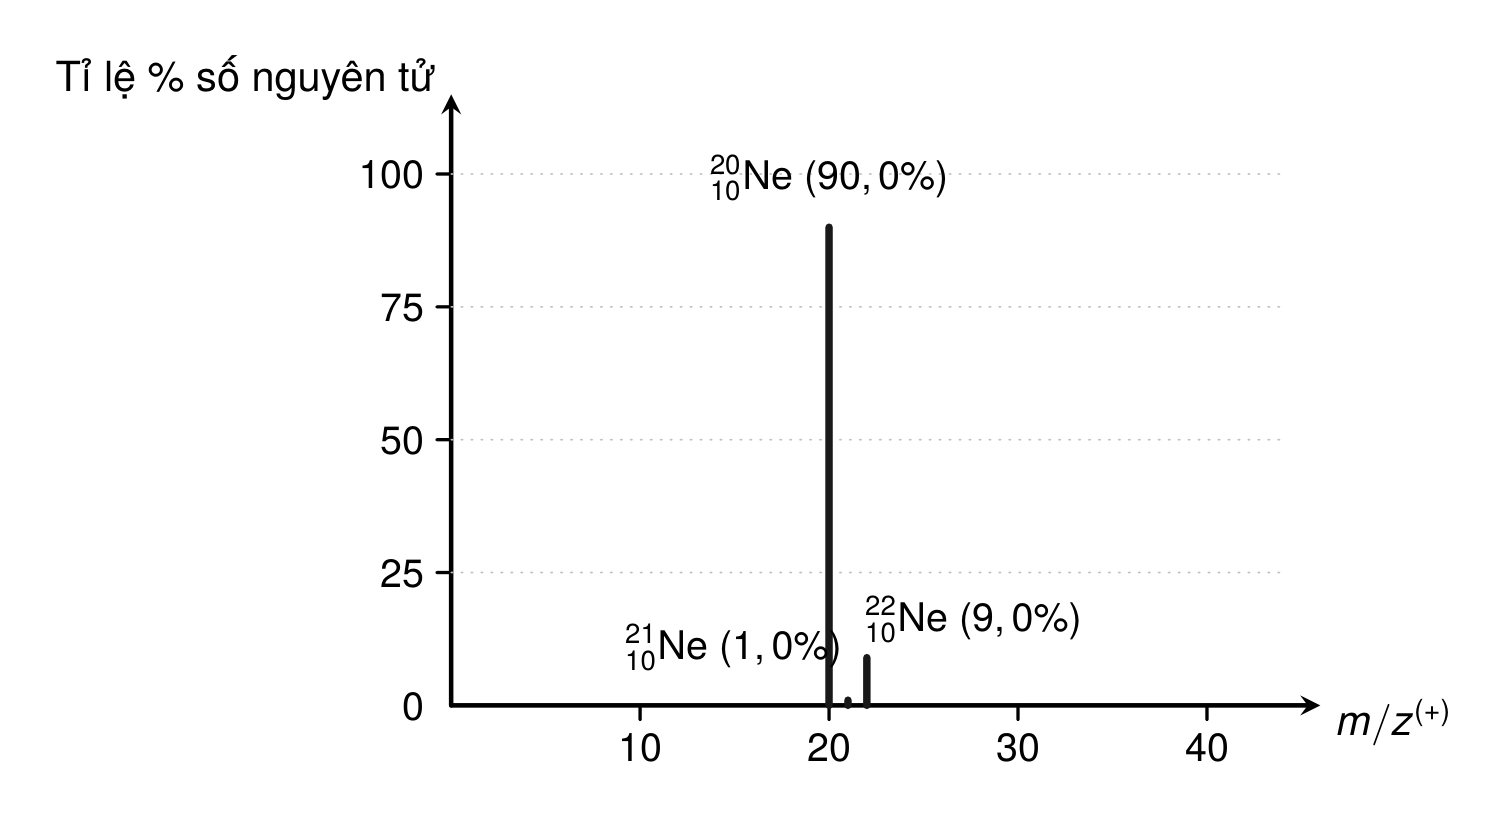
\includegraphics[width=8.5cm]{images_hoa10/pho_khoi_luong_neon_1201.png}
\end{center}
a) Tính nguyên tử khối trung bình của Neon (kết quả làm tròn đến hàng phần trăm).\\
b) Tính số nguyên tử của mỗi loại đồng vị còn lại khi có 1 nguyên tử $^{21}_{10}\ce{Ne}$ (kết quả làm tròn đến hàng đơn vị).\\
c) Tính thể tích của 10 gam Ne ở điều kiện chuẩn ($25^\circ\text{C}$, 1 bar) (kết quả làm tròn đến hàng phần mười).

\loigiai{
Dựa vào phổ khối lượng:\\
$^{20}_{10}\ce{Ne}$ chiếm 90,0\%; $^{21}_{10}\ce{Ne}$ chiếm 1,0\%; $^{22}_{10}\ce{Ne}$ chiếm 9,0\%.\\
a) Nguyên tử khối trung bình của Neon:
$$\overline{A}_{\ce{Ne}} = \frac{20 \times 90,0 + 21 \times 1,0 + 22 \times 9,0}{100} = \frac{2019}{100} = 20,19. \hfill \textit{(0,4 điểm)}$$
b) Tỉ lệ số nguyên tử của ba đồng vị:
$$N(^{20}\ce{Ne}) : N(^{21}\ce{Ne}) : N(^{22}\ce{Ne}) = 90,0 : 1,0 : 9,0 = 90 : 1 : 9.$$
Khi có 1 nguyên tử $^{21}_{10}\ce{Ne}$ thì có tương ứng:
- 90 nguyên tử $^{20}_{10}\ce{Ne}$.
- 9 nguyên tử $^{22}_{10}\ce{Ne}$. \hfill \textit{(0,3 điểm)}\\
c) Số mol của 10 gam Ne:
$$n_{\ce{Ne}} = \frac{10}{20,19} \approx 0,4953\text{ mol.}$$
Ở điều kiện chuẩn ($25^\circ\text{C}$, 1 bar):
$$V_{\ce{Ne}} = 0,4953 \times 24,79 \approx 12,278 \approx 12,3\text{ (lít)}. \hfill \textit{(0,3 điểm)}$$
}
\end{ex}
\begin{ex}
\textbf{(1,0 điểm)} Nguyên tố R thuộc nhóm A trong bảng tuần hoàn. Nguyên tử R có tổng số electron ở các phân lớp s là 7 và tổng số electron ở lớp ngoài cùng là 1.\\
a) Viết cấu hình electron đầy đủ của nguyên tử R. Dự đoán tính chất hóa học cơ bản của nguyên tố R (kim loại hay phi kim) và giải thích.\\
b) Phân tử $\ce{R2XY4}$ có tổng số hạt proton là 86. Biết nguyên tố X và Y thuộc cùng một nhóm A và ở hai chu kì liên tiếp trong bảng tuần hoàn. Hãy xác định số hiệu nguyên tử của X và Y.

\loigiai{
a) Xác định nguyên tố R:\\
- R thuộc nhóm A, có tổng số electron ở các phân lớp s là 7: $\ce{1s^2 2s^2 3s^2 4s^1}$ (tổng số electron s là $2 + 2 + 2 + 1 = 7$).\\
- Lớp ngoài cùng (lớp 4) có 1 electron ($4s^1$).\\
$\implies$ Cấu hình electron đầy đủ của R: $\ce{1s^2 2s^2 2p^6 3s^2 3p^6 4s^1}$ (hay $[\ce{Ar}]\ce{4s^1}$).\\
Nguyên tử R có $Z = 19$ (Potassium - $\ce{K}$).\\
- Dự đoán tính chất: R là một kim loại mạnh (kim loại kiềm điển hình).\\
Giải thích: Nguyên tử R có 1 electron ở lớp ngoài cùng, bán kính nguyên tử lớn, năng lượng ion hóa nhỏ nên rất dễ nhường đi 1 electron này để đạt cấu hình bền vững của khí hiếm Argon ($\ce{R \to R^+ + 1e}$). \hfill \textit{(0,5 điểm)}\\
b) Xác định số hiệu nguyên tử của X và Y:\\
- Phân tử $\ce{R2XY4}$ có tổng số proton là 86:
$$2Z_R + Z_X + 4Z_Y = 86 \implies 2 \times 19 + Z_X + 4Z_Y = 86 \implies Z_X + 4Z_Y = 48.\quad (*)$$
- X và Y thuộc cùng nhóm A và ở hai chu kì liên tiếp trong bảng tuần hoàn:\\
Vì $Z_X + 4Z_Y = 48$ nên $Z_Y < 12 \implies$ Y thuộc chu kì nhỏ (chu kì 2 hoặc 3). Hai nguyên tố cùng nhóm A ở hai chu kì nhỏ hơn kém nhau 8 proton: $|Z_X - Z_Y| = 8$.\\
+ TH1: $Z_Y = Z_X + 8 \implies Z_X + 4(Z_X + 8) = 48 \implies 5Z_X = 16 \implies Z_X = 3,2$ (loại).\\
+ TH2: $Z_X = Z_Y + 8 \implies (Z_Y + 8) + 4Z_Y = 48 \implies 5Z_Y = 40 \implies Z_Y = 8 \implies Z_X = 16$.\\
- Kiểm tra: Y ($Z = 8$): chu kì 2, nhóm VIA (Oxygen - $\ce{O}$); X ($Z = 16$): chu kì 3, nhóm VIA (Sulfur - $\ce{S}$). Thỏa mãn cùng nhóm VIA ở hai chu kì liên tiếp 2 và 3 (hợp chất là $\ce{K2SO4}$).\\
Vậy: Số hiệu nguyên tử của X là 16 (Sulfur) và số hiệu nguyên tử của Y là 8 (Oxygen). \hfill \textit{(0,5 điểm)}
}
\end{ex}
\vspace{6pt}
\begin{center}
\textbf{---------- HẾT ----------}\\
\textit{\small - Thí sinh không được sử dụng tài liệu.\\
- Cán bộ coi thi không giải thích gì thêm.}
\end{center}
\end{document}
